%!TEX program = xelatex
\documentclass[a4paper,12pt,fontset=ubuntu]{ctexart}

% --- 页面设置 ---
\usepackage[top=2.5cm, bottom=2.5cm, left=2.5cm, right=2.5cm]{geometry}
\usepackage{fancyhdr}
\usepackage{lastpage}

% --- 字体和段落 ---
\usepackage{fontspec}
\setmainfont{Times New Roman}
% ctexart 已经设置了中文宋体作为主要字体
% 如果需要更精细控制，可以使用 \setCJKmainfont{SimSun} 等

\usepackage{indentfirst} % 首行缩进
\setlength{\parindent}{2em}
\linespread{1.25} % 约等于单倍行距

% --- 标题格式 ---
\usepackage{titlesec}

% 一级标题: "第X部分" 黑体三号(16pt), 居中
\titleformat{\section}[block]{\centering\zihao{3}\heiti}{第\thesection 部分}{1em}{}
\titlespacing{\section}{0pt}{24pt}{16pt}
% 每次新的一节重置计数器 (公式、图、表) - LaTeX 默认按 section 编号需要 amsmath 和 caption 配置，这里手动处理可能比较复杂，
% 通常 LaTeX 习惯是 1.1, 1.2 连续编号，或者按 section 重置。
% 这里我们使用 chngcntr 包来实现按 section重置
\usepackage{chngcntr}
\counterwithin{figure}{section}
\counterwithin{table}{section}
\counterwithin{equation}{section}

% 二级标题: 黑体四号(14pt)
\titleformat{\subsection}{\zihao{4}\heiti}{\thesubsection}{1em}{}
\titlespacing{\subsection}{0pt}{12pt}{6pt}

% 三级标题: 小四宋体(12pt)
\titleformat{\subsubsection}{\zihao{-4}\songti}{\thesubsubsection}{1em}{}
\titlespacing{\subsubsection}{0pt}{6pt}{3pt}

% --- 图表和公式配置 ---
\usepackage{graphicx}
\usepackage{caption}
\usepackage{float}
\usepackage{booktabs} % 更好的表格线
\usepackage{amsmath}
\usepackage{amssymb}
\usepackage{cases} % 用于 cases 环境

% 图表标题格式: 五号宋体加粗
\DeclareCaptionFont{fivebold}{\zihao{5}\songti\bfseries}
\captionsetup{font=fivebold, labelsep=quad}
% 图表编号格式: 1-1
\renewcommand{\thefigure}{\thesection-\arabic{figure}}
\renewcommand{\thetable}{\thesection-\arabic{table}}
\renewcommand{\theequation}{\thesection-\arabic{equation}}


% --- 页眉页脚 ---
\pagestyle{fancy}
\fancyhf{} % 清空当前页眉页脚
\cfoot{\zihao{5}\songti 第 \thepage 页 共 \pageref{LastPage} 页}
\renewcommand{\headrulewidth}{0pt} % 移除页眉线

% --- 其他宏包 ---
\usepackage{hyperref} % 超链接，通常放在最后
\hypersetup{
    colorlinks=true,
    linkcolor=black,
    filecolor=black,
    urlcolor=black,
    citecolor=black,
}

% --- 自定义命令 ---
\newcommand{\keywords}[1]{%
    \vspace{6pt}
    \noindent{\zihao{5}\songti\textbf{关键词：}#1}
}


\begin{document}

% ============================================================
% 第 1 页: 封面
% ============================================================
\begin{titlepage}
    \centering
    \vspace*{1cm}
    
    {\zihao{4}\heiti 2026 年英特尔杯大学生电子设计竞赛嵌入式系统专题邀请赛}
    
    \vspace{0.3cm}
    
    {\zihao{4} 2026 Intel Cup Undergraduate Electronic Design Contest}
    
    \vspace{0.15cm}
    
    {\zihao{4} - Embedded System Design Invitational Contest}
    
    \vspace{1.5cm}
    
    {\zihao{2}\kaishu\bfseries 初选项目设计方案书}
    
    \vspace{3cm}
    
    % TODO: 插入赛事 LOGO 图片
    % \includegraphics[width=4cm]{esic_logo.png}
    % {\zihao{-4} Intel Cup Embedded System Design Contest}
    
    \vspace{2cm}
    
    {\zihao{4}\kaishu\bfseries 项目题目：\underline{\hspace{1em}LabGuardian：基于边缘AI的智能实验助教系统\hspace{1em}}}
    
    \vspace{2cm}
    
    {\zihao{4}\kaishu
    \renewcommand{\arraystretch}{1.5}
    \begin{tabular}{rl}
        学生姓名：& \underline{\makebox[6cm]{}} \\
        指导教师：& \underline{\makebox[6cm]{}} \\
        参赛学校：& \underline{\makebox[6cm]{}} \\
    \end{tabular}
    }
    
    \vfill
\end{titlepage}

% ============================================================
% 第 2 页: 题目 + 摘要
% ============================================================
\setcounter{page}{1} % 假设从这里开始计数，或者从目录开始

\begin{center}
    {\zihao{3}\heiti\bfseries LabGuardian：基于边缘AI的智能理工科实验助教系统}
\end{center}

\vspace{1.5cm}

\begin{center}
    {\zihao{3}\heiti\bfseries 摘要}
\end{center}

\vspace{12pt}

% 摘要正文
\noindent
（摘要正文待填写。五号宋体，首行缩进二个字，单倍行距。）

\keywords{边缘AI，旋转目标检测，电路拓扑分析，异构计算，Intel OpenVINO，实验教学}

\newpage

% ============================================================
% 第 3 页: 目录 (可选)
% ============================================================

\renewcommand{\contentsname}{\centerline{\zihao{3}\heiti\bfseries 目\hspace{2em}录}}
\tableofcontents

\newpage

% ============================================================
% 第一部分  项目背景
% ============================================================

\section{项目背景}
\label{sec:background}

\subsection{行业痛点分析}

在高等理工科教育体系中，电路分析、模拟/数字电子技术等基础实验课程是培养学生工程素养的关键环节。然而，当前实验教学在“规模化普及”与“精细化指导”之间存在难以调和的结构性矛盾，具体表现在以下三个层面。

\textbf{（1）师生资源配比严重失衡。}根据教育部《2024年全国教育事业发展统计公报》，我国普通高校专任教师与在校学生比约为 1:18，而在实验教学环节，尤其是电子、电气类基础实验课程中，单班实验师生比普遍达到 1:30 甚至更高。这意味着当学生在面包板接线中遇到故障时，平均需要等待 5–10 分钟才能获得教师介入。这种“指导真空期”不仅消磨了学生的探索热情，也迫使教师将大量精力耗费在排查低级接线错误上，无法聚焦于更有价值的原理讲解与思维引导。

\textbf{（2）理论与工程的认知鸿沟。}初学者难以将抽象的二维电路原理图高效映射至三维的物理面包板空间。这种“空间思维转换”的高门槛导致试错成本激增：据多所高校实验中心统计，每学期因电源极性反接、短路等操作失误导致的芯片与传感器损坏率高达 8\%–15\%，这既增加了实验室运维成本，也影响了教学进度。更重要的是，学生往往在“把实验做完”与“把原理吃透”之间选择了前者，导致实践教学的育人价值大打折扣。

\textbf{（3）现有辅助手段的交互局限。}目前高校常用的实验辅助工具主要分为两类：一是以 Multisim、Proteus 为代表的离线仿真软件，其优势在于仿真精度高，但无法感知学生的实物接线情况，仿真与现实“两张皮”；二是以数据采集卡、数字示波器为代表的被动式测量仪器，其只能显示电气参数，无法从视觉层面识别“哪根线接错了”。学生迫切需要一种能够实时感知物理电路状态、提供精准纠错引导的智能辅助系统。

与此同时，我们调研发现，目前国内外尚无针对面包板电路实验场景的开源 AI 辅助教学项目。现有的教育 AI 研究多聚焦于自然语言处理（智能批改、自动出题）或纯软件仿真，尚无系统将计算机视觉、图论分析与大语言模型融合，应用于“看见物理电路$\rightarrow$理解拓扑连接$\rightarrow$给出纠错建议”这一端到端闭环的。这正是 LabGuardian 项目的创新空间所在。

\subsection{竞赛契合度与 Intel 平台优势}

本项目与英特尔杯嵌入式 AI 专题赛的核心要求高度契合。竞赛强调“基于 Intel 异构计算平台解决实际问题”，而 LabGuardian 的多模态感知与多级推理负载恰好需要 Intel Core Ultra 的异构算力解耦能力来支撑。具体而言，本项目采用“专芯专用、负载解耦”的异构调度策略：

\textbf{（1）视觉感知任务$\rightarrow$ iGPU (Intel Arc)。}YOLOv8-OBB 旋转目标检测模型通过 OpenVINO 部署于集成显卡，利用 GPU 并行浮点计算能力实现毫秒级推理。若依赖纯 CPU 推理，相同模型的帧率仅为个位数，无法满足实时性要求。

\textbf{（2）知识推理任务$\rightarrow$ NPU/CPU。}大语言模型（Qwen2.5-1.5B INT4）利用 NPU 的低功耗持续矩阵运算能力实现离线问答，避免与 YOLO 推理争抐显存资源。

\textbf{（3）逻辑仲裁任务$\rightarrow$ CPU (P-Core)。}图论分析、VF2++ 子图同构等复杂分支计算任务交由性能核处理，充分发挥其复杂分支与操作系统调度能力。

这种“三路并行”的异构架构是传统单片机 (MCU) 或单一 GPU 平台无法实现的。Intel Core Ultra 的 CPU + iGPU + NPU 三单元协同架构，为本项目提供了理想的硬件基底，也充分体现了竞赛平台的设计初衷——让参赛者在真实的嵌入式场景中探索异构 AI 的工程实践。

\subsection{应用前景}

LabGuardian 的核心应用价值可从以下三个维度展开。

\textbf{（1）学习范式跃迁：从“事后纠错”到“过程引导”。}传统实验模式下，学生接完电路后才知道对错，学习反馈回路过长。LabGuardian 将检测与引导前置到接线过程中，学生每插入一个元件即可获得实时反馈，帮助其从“把实验做完”升级为“把原理吃透”，真正实现实践教学的育人目标。

\textbf{（2）资源效率优化：降低设备损耗与师资压力。}系统作为“第一道防线”拦截大部分基础连接错误，显著降低因短路、反接等引起的芯片损坏率，减少实验室耗材开支。同时，教师得以从重复性的接线排查工作中释放出来，将更多精力投入到原理讲解、创新实验设计等高价值的教学活动中。

\textbf{（3）边缘部署保障数据合规与全离线可用。}LabGuardian 的全部推理计算均在 DK-2500 边缘设备上完成，视频数据不出域。这一特性使系统天然适配屏蔽实验室、断网考试环境等弱网场景，也符合校园数据安全与学生隐私保护要求。

从更广泛的视角来看，随着教育部持续推动“AI+教育”融合创新，及 Intel 等主流芯片厂商将 NPU 作为标配纳入消费级处理器，边缘 AI 辅助教学有望从实验室向课堂、实训基地乃至职业教育等场景扩展。LabGuardian 所积累的“视觉感知$\rightarrow$图论推理$\rightarrow$智能问答”技术框架，可复用于电子装配质检、PCB 焦点审查等工业场景，具备良好的技术迁移性与产业化潜力。


% ============================================================
% 第二部分  项目设计方案
% ============================================================

\section{项目设计方案}
\label{sec:design}

\subsection{研究开发内容}

本系统定位为部署在每个实验台上的“全能电子助教”，具备“看、想、说”三大核心能力：

\textbf{（1）实时电路纠错。}摄像头实时监控面包板，自动识别元器件布局与连线，将识别到的电路拓扑与标准模板进行图同构对比，检测短路、断路、极性反接等错误，在屏幕上高亮标注错误位置。

\textbf{（2）智能器件问答。}集成离线大语言模型（LLM），学生可通过自然语言询问元器件参数、电路原理等问题，系统结合当前检测上下文（元件清单、连接状态）生成结构化回答。

\textbf{（3）电路可视化标注。}在实时视频流上叠加虚拟连线标注，呈现电流路径与纠错提示，实现“所见即所得”的直观教学引导。

\subsection{系统架构}

系统采用“感知—认知—逻辑”（See-Think-Control）三位一体分层架构，精确映射 Intel Core Ultra 异构硬件特性。软件分为四个核心模块，如图 \ref{fig:arch} 所示。

% TODO: 插入系统架构图
\begin{figure}[htbp]
    \centering
    % 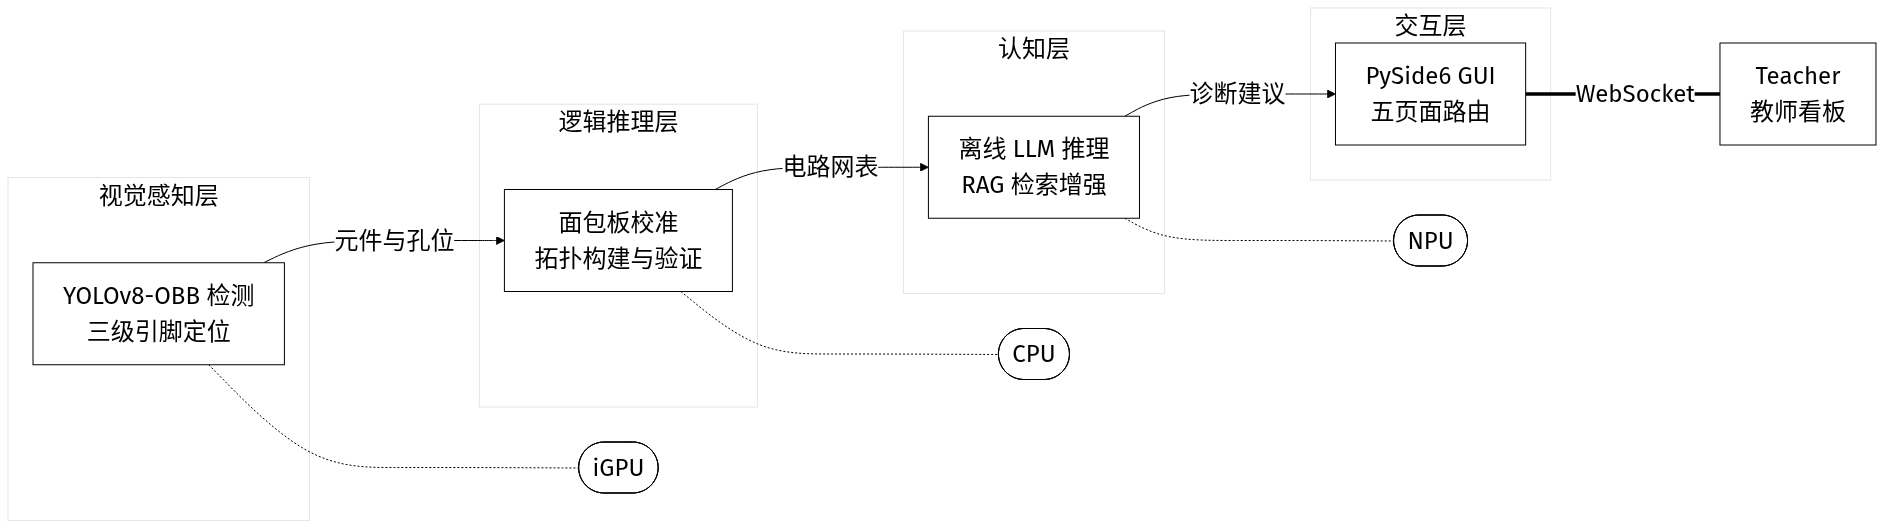
\includegraphics[width=0.9\textwidth]{pictures/system_architecture.png}
    \caption{系统总体架构图}
    \label{fig:arch}
\end{figure}

\subsubsection{视觉感知层（Vision）$\rightarrow$ iGPU}

基于 YOLOv8-OBB（旋转目标检测）模型，识别面包板上 7 类电子元器件（电阻、LED、电容、二极管、导线、IC 芯片、按钮）。选择 OBB 而非传统水平框（HBB），是因为面包板上元件多为倾斜或垂直插入，旋转框能精确描述元件角度与长宽比，有效解决密集元件间的 IoU 粘连问题。OBB 检测结果结构化为 \texttt{Detection} 数据类，包含类别、置信度、OBB 角点、推算引脚坐标等信息。

如图 \ref{fig:yolo-demo} 所示，系统可对实验台上的多种元器件进行实时检测与标注。

\begin{figure}[htbp]
    \centering
    % 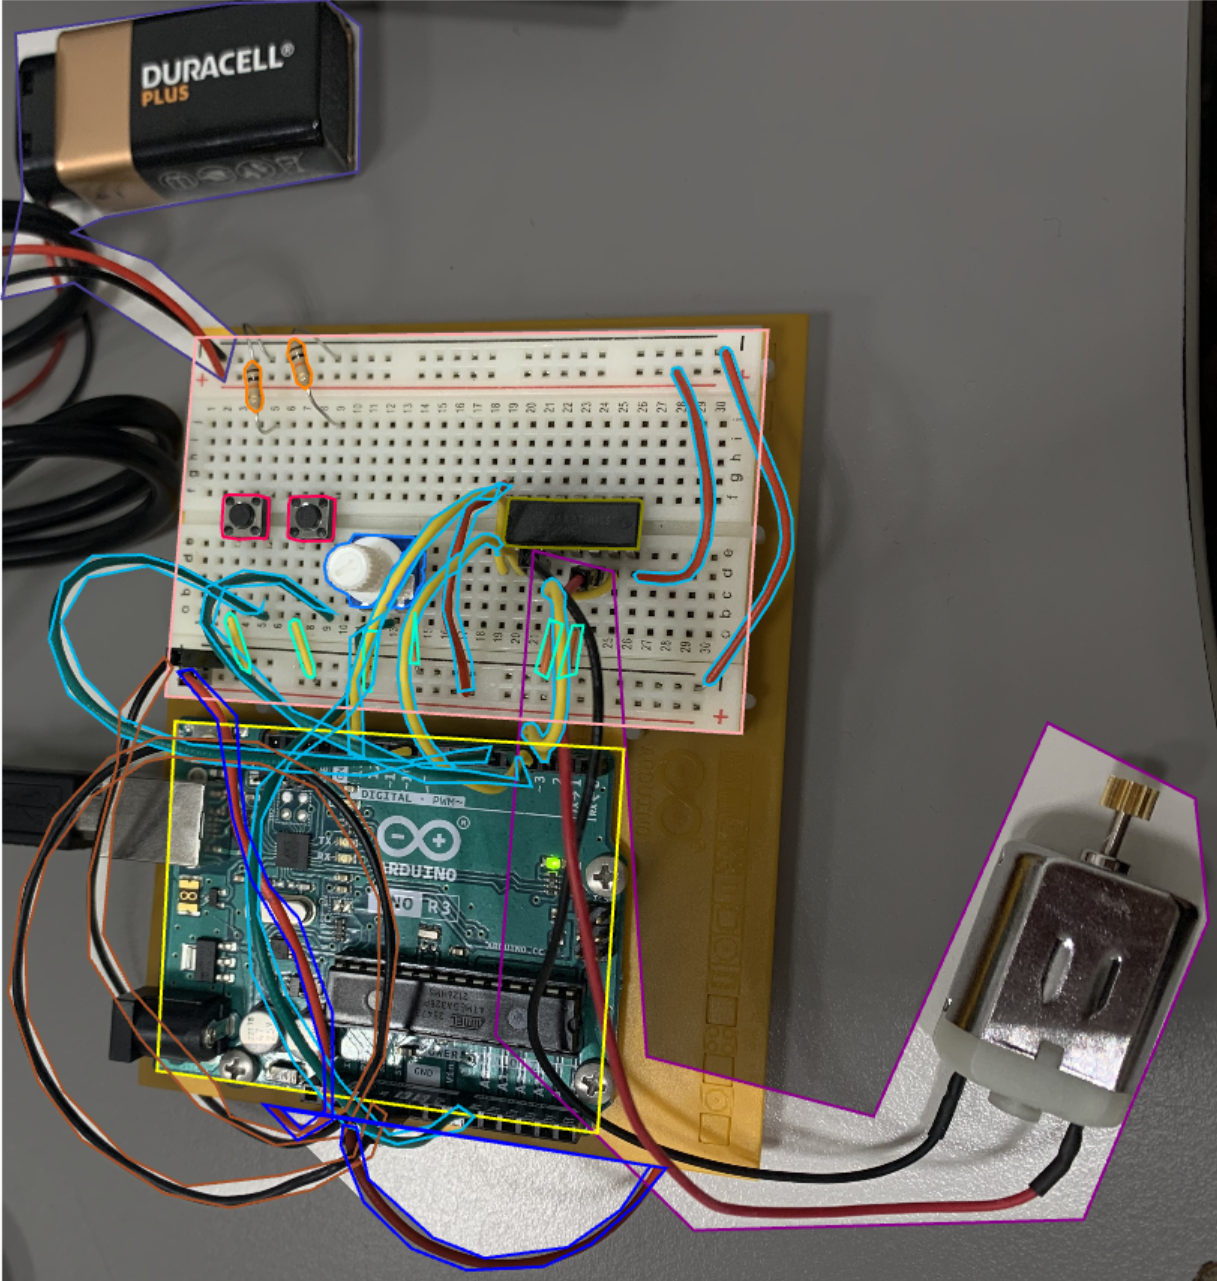
\includegraphics[width=0.75\textwidth]{pictures/yolo_demo.png}
    % TODO: 上传图片 pictures/yolo_demo.png 后取消注释
    \fbox{\parbox{0.75\textwidth}{\centering\vspace{2cm}图片占位符：yolo\_demo.png\vspace{2cm}}}
    \caption{YOLOv8-OBB 元器件检测效果示例}
    \label{fig:yolo-demo}
\end{figure}

为提高检测稳定性，系统引入多帧滑窗投票稳定器（DetectionStabilizer）。设窗口大小为 $W$，每一帧的检测结果通过 IoU 匹配关联到已有轨迹，只有获得 $k$ 票以上的检测结果才被确认为有效：

\begin{equation}
\text{confirmed}(d) = \begin{cases}
  \text{True} & \text{if } \sum_{i=1}^W \mathbb{I}[\text{IoU}(d, d_i) > \tau] \ge k, \\
  \text{False} & \text{otherwise}
\end{cases}
\label{eq:stabilizer}
\end{equation}

其中 $\tau$ 为 IoU 阈值（默认 0.5），$k$ 为最小票数（默认 3）。该机制有效抑制单帧误检与闪烁。

\subsubsection{逻辑推理层（Logic）$\rightarrow$ CPU}

逻辑层实现从“像素坐标”到“电气连接关系”的关键转换，包含三个核心子模块。

\textbf{面包板校准器（Calibrator）。}实现五级鲁棒孔洞检测管线——Level 1: \texttt{cv2.findCirclesGrid} 对称圆网格检测；Level 2: 多参数 \texttt{SimpleBlobDetector} 集成检测；Level 3: \texttt{HoughCircles} 补漏；Level 4: 轮廓几何分析兜底；最终通过 NMS 去重与 RANSAC 网格拟合剔除离群点并补全缺失孔位。如图 \ref{fig:breadboard} 所示，面包板的孔洞网格结构为后续引脚映射提供基准。

\begin{figure}[htbp]
    \centering
    % 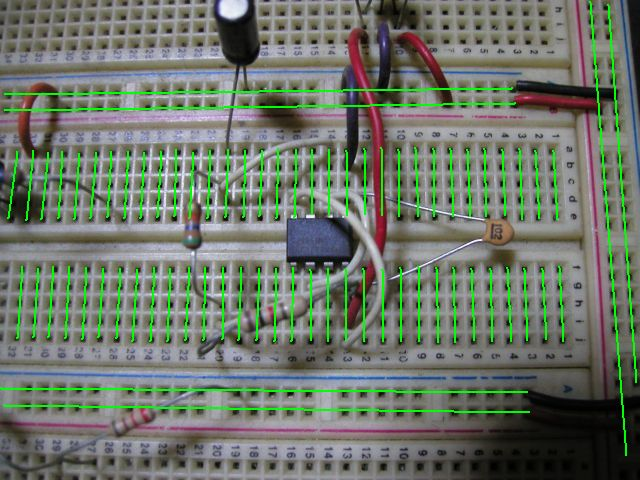
\includegraphics[width=0.6\textwidth]{pictures/breadboard_structure.jpg}
    % TODO: 上传图片 pictures/breadboard_structure.jpg 后取消注释
    \fbox{\parbox{0.6\textwidth}{\centering\vspace{2cm}图片占位符：breadboard\_structure.jpg\vspace{2cm}}}
    \caption{面包板孔洞网格结构与导通规则}
    \label{fig:breadboard}
\end{figure}

\textbf{电路分析器（CircuitAnalyzer）。}基于 NetworkX 图论引擎，将元件检测结果转化为电路拓扑图 $G = (V, E)$。顶点集 $V$ 为电气节点（由面包板导通规则合并），边集 $E$ 为元器件连接。根据面包板导通规则（纵向 5 孔导通、电源轨横向导通）构建电气连接图，生成标准 Netlist 网表。集成极性解析器（PolarityResolver），利用 OBB 旋转角度与元件几何特征推断二极管/LED 正负极、三极管 B/C/E 引脚，无额外机器学习开销。

\textbf{电路验证器（CircuitValidator）。}采用 VF2++ 子图同构算法实现标准电路与实测电路的精确对比。给定标准电路图 $G_{\text{ref}}$ 与实测电路图 $G_{\text{det}}$，验证器求解子图同构映射 $\phi: V(G_{\text{ref}}) \rightarrow V(G_{\text{det}})$，使得：

\begin{equation}
\forall (u, v) \in E(G_{\text{ref}}): (\phi(u), \phi(v)) \in E(G_{\text{det}})
\label{eq:vf2}
\end{equation}

若同构映射不存在，验证器进入三级诊断流程：元件类型差异分析、连接拓扑差异分析、极性/引脚赋值差异分析，输出结构化诊断报告（缺失元件、多余元件、极性反接、引脚错位、电源网络异常等）。

\subsubsection{认知层（Cognition）$\rightarrow$ NPU/CPU}

部署离线双引擎，确保断网条件下提供智能问答：

\begin{itemize}
    \item \textbf{主引擎 — 本地推理。}使用 \texttt{openvino\_genai} 库在 NPU/CPU 上运行 Qwen2.5-1.5B-Instruct INT4 量化模型，完全离线；
    \item \textbf{兜底引擎 — 规则模板。}基于预设模板的规则引擎，零依赖兜底，保证基本纠错建议不中断。
\end{itemize}

系统完全离线运行，将检测上下文（元件清单、置信度、风险事件）注入 LLM 提示词，输出结构化建议（现象/证据/原因/下一步/风险），并对高风险建议启用白名单过滤，彻底消除数据出域风险。

\subsubsection{交互层（Interaction）$\rightarrow$ PySide6 GUI}

基于 PySide6（Qt6）构建 PyDracula 风格暗色主题界面，采用自定义无边框标题栏 + 侧边栏导航 + \texttt{QStackedWidget} 五页面路由（主面板/视频检测/AI 助手/电路验证/设置）。核心线程采用 \texttt{QThread} + 信号槽机制分离：\texttt{VideoWorker} 负责视频采集与 YOLO 推理，\texttt{LLMWorker} 负责异步问答，\texttt{ModelLoaderWorker} 负责模型加载，确保 UI 始终流畅。

% TODO: 插入 GUI 截图
\begin{figure}[htbp]
    \centering
    % \includegraphics[width=0.85\textwidth]{pictures/gui_screenshot.png}
    \caption{LabGuardian 用户界面截图}
    \label{fig:gui}
\end{figure}

\subsection{技术关键及主要特色}

\textbf{（1）OBB 旋转检测解决密集布线场景。}传统水平框在面包板场景中引入大量背景噪声，导致引脚粘连。OBB 提供旋转角度参数 $\theta$，精确分割细长导线与倾斜电阻，并从 OBB 几何直接推算元件两端引脚像素坐标。如图 \ref{fig:obb-chip} 所示，系统可对密集排布的芯片引脚进行精确检测。

\begin{figure}[htbp]
    \centering
    % 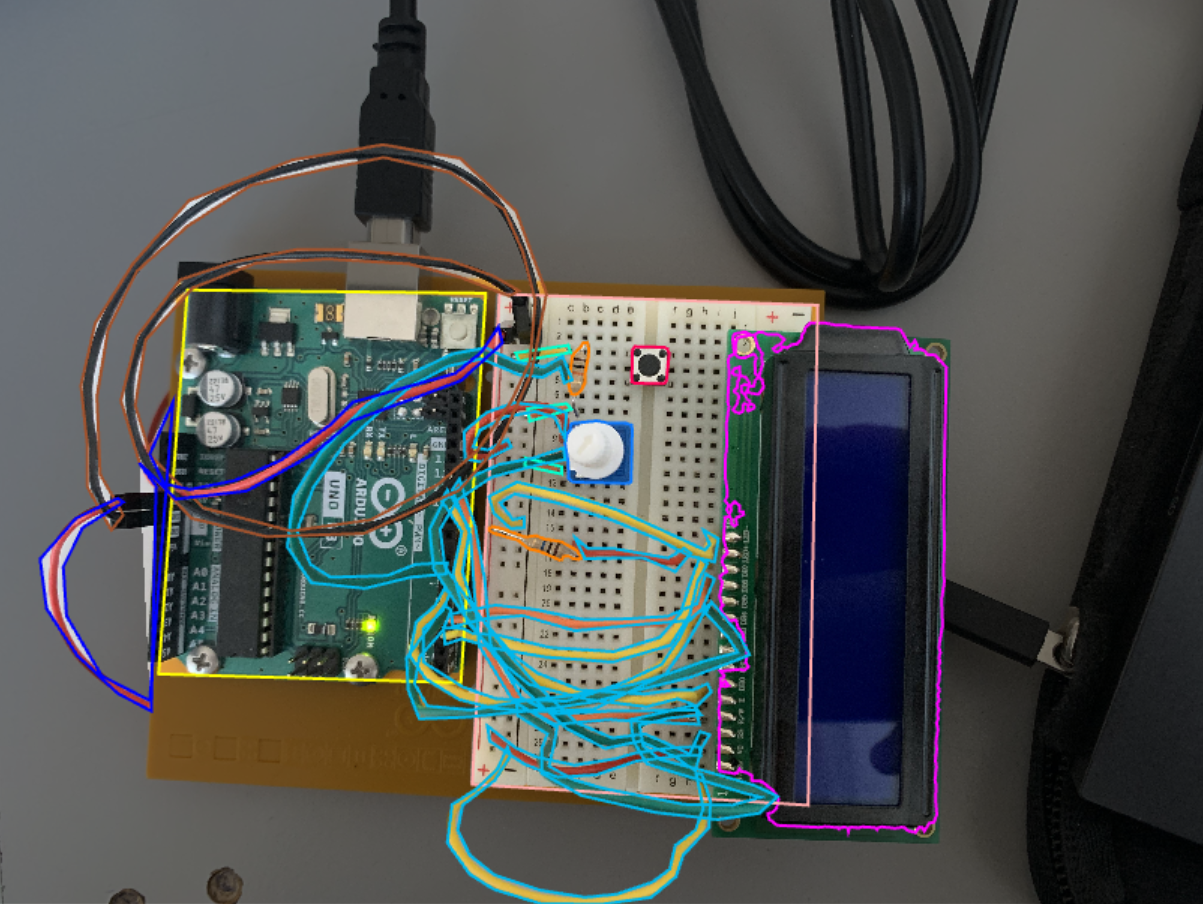
\includegraphics[width=0.7\textwidth]{pictures/yolo_inference_chip.png}
    % TODO: 上传图片 pictures/yolo_inference_chip.png 后取消注释
    \fbox{\parbox{0.7\textwidth}{\centering\vspace{2cm}图片占位符：yolo\_inference\_chip.png\vspace{2cm}}}
    \caption{OBB 检测在密集元件场景下的效果}
    \label{fig:obb-chip}
\end{figure}

\textbf{（2）五级面包板校准管线。}针对孔洞检测在不同光照/面包板型号下的鲁棒性问题，设计了从精确到模糊的五级检测级联，配合 CLAHE 光照归一化预处理，最终通过 RANSAC 网格拟合统一输出标准化孔位坐标。引脚到孔位的映射误差控制在 $\pm 1$ 格以内。

\textbf{（3）极性感知的拓扑验证。}在传统的拓扑同构对比基础上，引入元件极性与引脚角色信息。系统不仅检测“少了一个 LED”，更能诊断“LED 接反了”或“三极管 B/C/E 接错”，参考 EDA 领域 LVS（Layout vs.\ Schematic）方法论。

\textbf{（4）三级 LLM 降级保证离线可用。}系统自动探测网络状态，按 Cloud $\rightarrow$ Local $\rightarrow$ Rule 顺序选择最优后端，切换对用户透明。本地 LLM 使用 OpenVINO GenAI 的 \texttt{LLMPipeline} 实现 NPU 加速推理。

\textbf{（5）全 Intel 原生工具链。}系统深度绑定 OpenVINO 生态：模型导出为 OpenVINO IR 格式，视觉推理走 iGPU 插件，LLM 推理走 NPU/CPU 插件，通过 NNCF 进行 INT4/INT8 量化压缩。

\subsection{预期目标}

本项目的关键性能指标（KPI）如表 \ref{tab:kpi} 所示。

\begin{table}[htbp]
    \centering
    \caption{LabGuardian 关键性能指标（KPI）}
    \label{tab:kpi}
    \begin{tabular}{c c l}
        \toprule
        \textbf{指标} & \textbf{目标值} & \textbf{说明} \\
        \midrule
        元器件识别率 & mAP@0.5 $\ge 80\%$ & 含遮挡与光照变化场景 \\
        端到端纠错延迟 & $< 200$ ms & 从图像采集到纠错反馈，含多帧稳定化 \\
        LLM 首字生成时间 & $< 3$ s & NPU 离线推理条件下 \\
        支持元器件种类 & $\ge 7$ 类 & 电阻/LED/电容/二极管/导线/IC/按钮 \\
        系统连续运行稳定性 & $\ge 2$ 小时 & 无崩溃、无内存泄漏 \\
        视频推理帧率 & $\ge 15$ FPS & 960p 分辨率，iGPU 推理 \\
        \bottomrule
    \end{tabular}
\end{table}


\subsection{项目实施方案与技术路线}

项目采用敏捷开发模式，分三个阶段推进，每阶段设置明确的交付里程碑。

\textbf{阶段 A：初选冲刺（2026.02—2026.03）。}完成数据采集与标注（200–300 张多环境面包板照片，7 类 OBB 标注）、YOLO 模型重新训练（yolov8s-obb, epochs=300, imgsz=960）、代码模块化重构（vision/logic/ai/gui 四模块架构）、PySide6 GUI 开发、设计方案书撰写。

\textbf{阶段 B：平台移植（2026.04—2026.05）。}在 DK-2500（Ubuntu）上搭建 OpenVINO 运行时环境，完成 YOLO 模型 OpenVINO 导出（FP16/INT8）并验证 iGPU 推理帧率（目标 $\ge 15$ FPS @ 960p），LLM 模型 NPU 部署（Qwen2.5-1.5B INT4），摄像头 V4L2 适配。

\textbf{阶段 C：功能打磨（2026.05—2026.06）。}开发一键纠错、安全预检（LED 无限流电阻告警）、电路仿真等差异化功能；完成系统性能调优、中英文报告撰写、压力测试（连续运行 2 小时、断网环境验证）。

技术路线的核心思路可概括为“PC 原型先行→DK-2500 无缝移植”：先在 x86 PC 上完成全链路功能验证，再利用 Intel Core Ultra 与 PC 的 x86 指令集兼容性，通过 OpenVINO 的硬件抽象层实现“代码不改、插件切换”的平滑迁移。

% TODO: 插入技术路线图
\begin{figure}[htbp]
    \centering
    % \includegraphics[width=0.9\textwidth]{pictures/tech_roadmap.png}
    \caption{项目技术路线图}
    \label{fig:roadmap}
\end{figure}

\subsection{进度安排}

\begin{table}[htbp]
    \centering
    \caption{项目进度安排}
    \label{tab:schedule}
    \begin{tabular}{c c l}
        \toprule
        \textbf{时间} & \textbf{阶段} & \textbf{核心交付物} \\
        \midrule
        2 月 10 日—3 月 5 日 & 数据与模型 & 标注数据集 + 训练模型 \\
        3 月 5 日—3 月 15 日 & 软件开发 & 模块化重构完成 + GUI \\
        3 月 15 日—3 月 25 日 & 初选材料 & 方案报告 + PPT + Demo 视频 \\
        4 月初—5 月中 & 平台移植 & DK-2500 全链路跑通 \\
        5 月中—6 月 30 日 & 功能打磨 & 最终作品 + 中英文报告 \\
        \bottomrule
    \end{tabular}
\end{table}

\subsection{异常处理与降级策略}

系统针对评审现场可能出现的异常情况设计了完整的降级路径，核心原则为“不断流、可恢复、可追溯”：

\begin{itemize}
    \item \textbf{摄像头异常。}掉线时自动重连并降低分辨率，多次重连失败后切换为静态图片分析模式。
    \item \textbf{OpenVINO 编译失败。}按 iGPU $\rightarrow$ NPU $\rightarrow$ CPU 级联回退，确保推理不中断。
    \item \textbf{帧率不足。}自动降低输入分辨率并启用抽帧（每 $n$ 帧取 1 帧），保证用户体验流畅。
    \item \textbf{LLM 延迟过大。}切换为规则模板优先模式，先输出基础纠错建议，LLM 响应到达后追加详细解释。
    \item \textbf{模型加载失败。}使用轻量级预训练模型（yolov8n）作为回退模型，确保基本检测能力不丢失。
\end{itemize}

所有异常事件均记录日志，支持事后回溯分析。

% ============================================================
% 第三部分  团队组成
% ============================================================

\section{团队组成}
\label{sec:team}

\subsection{团队成员组成}

% TODO: 填写正文

\subsection{成员特长与分工}

% TODO: 填写正文

\end{document}
